\documentclass[xcolor=dvipsnames]{beamer}

\usepackage[font=scriptsize,labelfont=bf]{caption}
\usepackage{listings}
\usepackage{url}
\usepackage{hyperref}
\usepackage{verb atim}
\usepackage{amsmath}
\usepackage{graphicx}
\usepackage{ragged2e}
\usepackage{tcolorbox}
\usepackage[dvipsnames]{xcolor}

\usetheme{Madrid}
%\useoutertheme[subsection=false]{smoothbars}

\AtBeginSection[]{
  \begin{frame}
  \vfill
  \centering
  \begin{beamercolorbox}[sep=8pt,center,shadow=true,rounded=true]{title}
    \usebeamerfont{title}\secname\par%
  \end{beamercolorbox}
  \vfill
  \end{frame}
}

\DeclareMathOperator*{\concat}{\mathbin\Vert}

\definecolor{UBCblue}{rgb}{0.04706, 0.13725, 0.26667} % UBC Blue (primary)
\definecolor{UBCgrey}{rgb}{0.3686, 0.5255, 0.6235} % UBC Grey (secondary)

\setbeamercolor{palette primary}{bg=UBCblue,fg=white}
\setbeamercolor{palette secondary}{bg=UBCblue,fg=white}
\setbeamercolor{palette tertiary}{bg=UBCblue,fg=white}
\setbeamercolor{palette quaternary}{bg=UBCblue,fg=white}
\setbeamercolor{structure}{fg=UBCblue} % itemize, enumerate, etc
\setbeamercolor{section in toc}{fg=UBCblue} % TOC sections
\renewcommand{\figurename}{Fig.}
%\logo{\includegraphics[height=1.2cm]{img/logo_di_black.png}}

% Override palette coloring with secondary
\setbeamercolor{subsection in head/foot}{bg=UBCgrey,fg=white}

\title[CBMIR for Pap Smear Images]{A Content-Based Medical Image Retrieval for Pap Smear Images with Generative Adversarial Networks and Nearest Neighbor}
\date{16 de Enero del 2023}
\author[CNF]{Camilo Núñez Fernández}
\institute[]{Departamento de Informática}

\begin{document}
	\begingroup 
        \setbeamertemplate{headline}{}
        \begin{frame}
            \titlepage
        \end{frame}
    \endgroup

    \begin{frame}{Problem - Background}
        \textbf{Objective disease}: Cervical Cancer \\\vspace{5mm}
        \textbf{Objective method}: Cervical smear images $\longrightarrow$ Papanicolaou Smear\\\vspace{5mm}
        \textbf{Some problems in Papanicolaou Smear Analysis}\\
        \begin{itemize}
            \item The screening process is expensive and time-consuming: this process take around 5 to 10 minutes based on the difficulty of cell. A cytothecnologist cannot analyse more than 70 samples on a day~\cite{Elsheikh2012}.
            \item The process also generate a large scale images that could affect the process with more delays in the workflow~\cite{9046839}.
        \end{itemize}\vspace{5mm}
        \textbf{Basic Solution}: A Content-Based Medical Image Retrieval~(CBMIR) service for Pap smear images, aimed to computer-aided diagnosis~(CAD).
    \end{frame}

    \begin{frame}{Problem - Definition}
        \textbf{Basic Solution}: A Content-Based Medical Image Retrieval~(CBMIR) service for Pap smear images, aimed to computer-aided diagnosis~(CAD).\\
        \vspace{5mm}
        \textbf{Involvements Basic Solution}:
        \begin{itemize}
            \item Inefficient retrieves (i e. bad solution for overlapping cells~\cite{Zhao2022}, absence of feedback-based options~\cite{9606873})
            \item Hard dependencies over the handcraft-annotations~\cite{Mller2004}.
            \item Losses in the semantic of the images~\cite{9046839}.
        \end{itemize}
        \vspace{5mm}
        \textbf{Complex Solution}: An \textbf{efficient} Content-Based Medical Image Retrieval~(CBMIR) with \textbf{robust and richness features vectors} for pap smear images.
    \end{frame}

    \begin{frame}{Related Work - Deep Learning - Classic Arqs}
       \begin{figure}
           \centering
           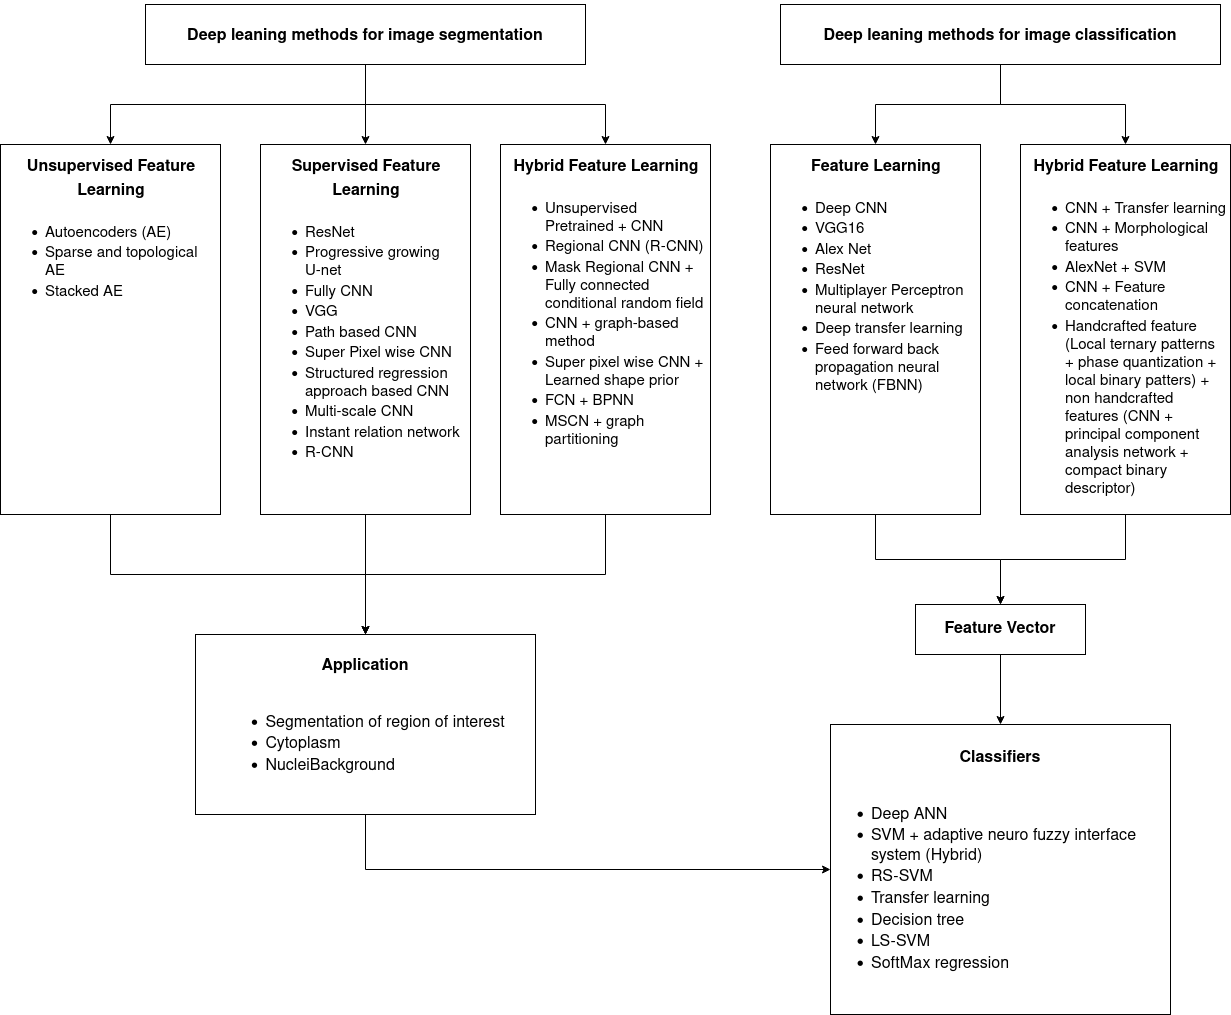
\includegraphics[width=0.79\paperwidth]{img/dl-algo.png}
       \end{figure}
    \end{frame}

    \begin{frame}{Related Work - Deep Learning - SOTA}
        \textbf{Generative Adversarial Networks - Cell-GAN~\cite{9513282}}
        \begin{itemize}
            \item Segmentation of cervical cell images
            \item Encoder-Decorder with double input generator
            \item Guide factor as prior
            \item Inception architecture discriminator
        \end{itemize}
        
        \begin{figure}
           \centering
           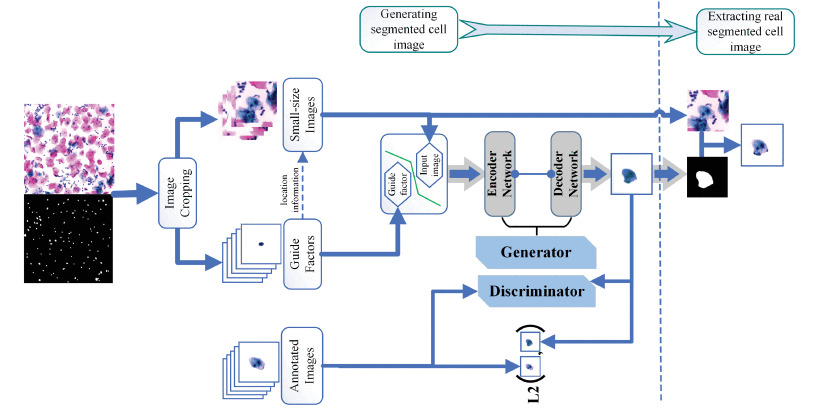
\includegraphics[width=0.7\paperwidth]{img/yang1-3104609-large.jpg}
       \end{figure}
    \end{frame}

    \begin{frame}{Related Work - Deep Learning - SOTA}
        \textbf{Tissue specific feature distillation network (TSFD-Net)~\cite{Ilyas2022}}
        \begin{itemize}
            \item Multi-task network: classification and segmentation (semantic and boundary)
            \item Three stages:
            \begin{enumerate}
                \item Feature distillation backbone with Mobile-Net-v2 and squeeze-excitation sub-network
                \item \textbf{Feature combinations} with cross-scale weighted feature fusion (CWFF) paths
                \item Interlinked decoders for semantic mask and boundary mask
            \end{enumerate}
        \end{itemize}
        
        \begin{figure}
           \centering
           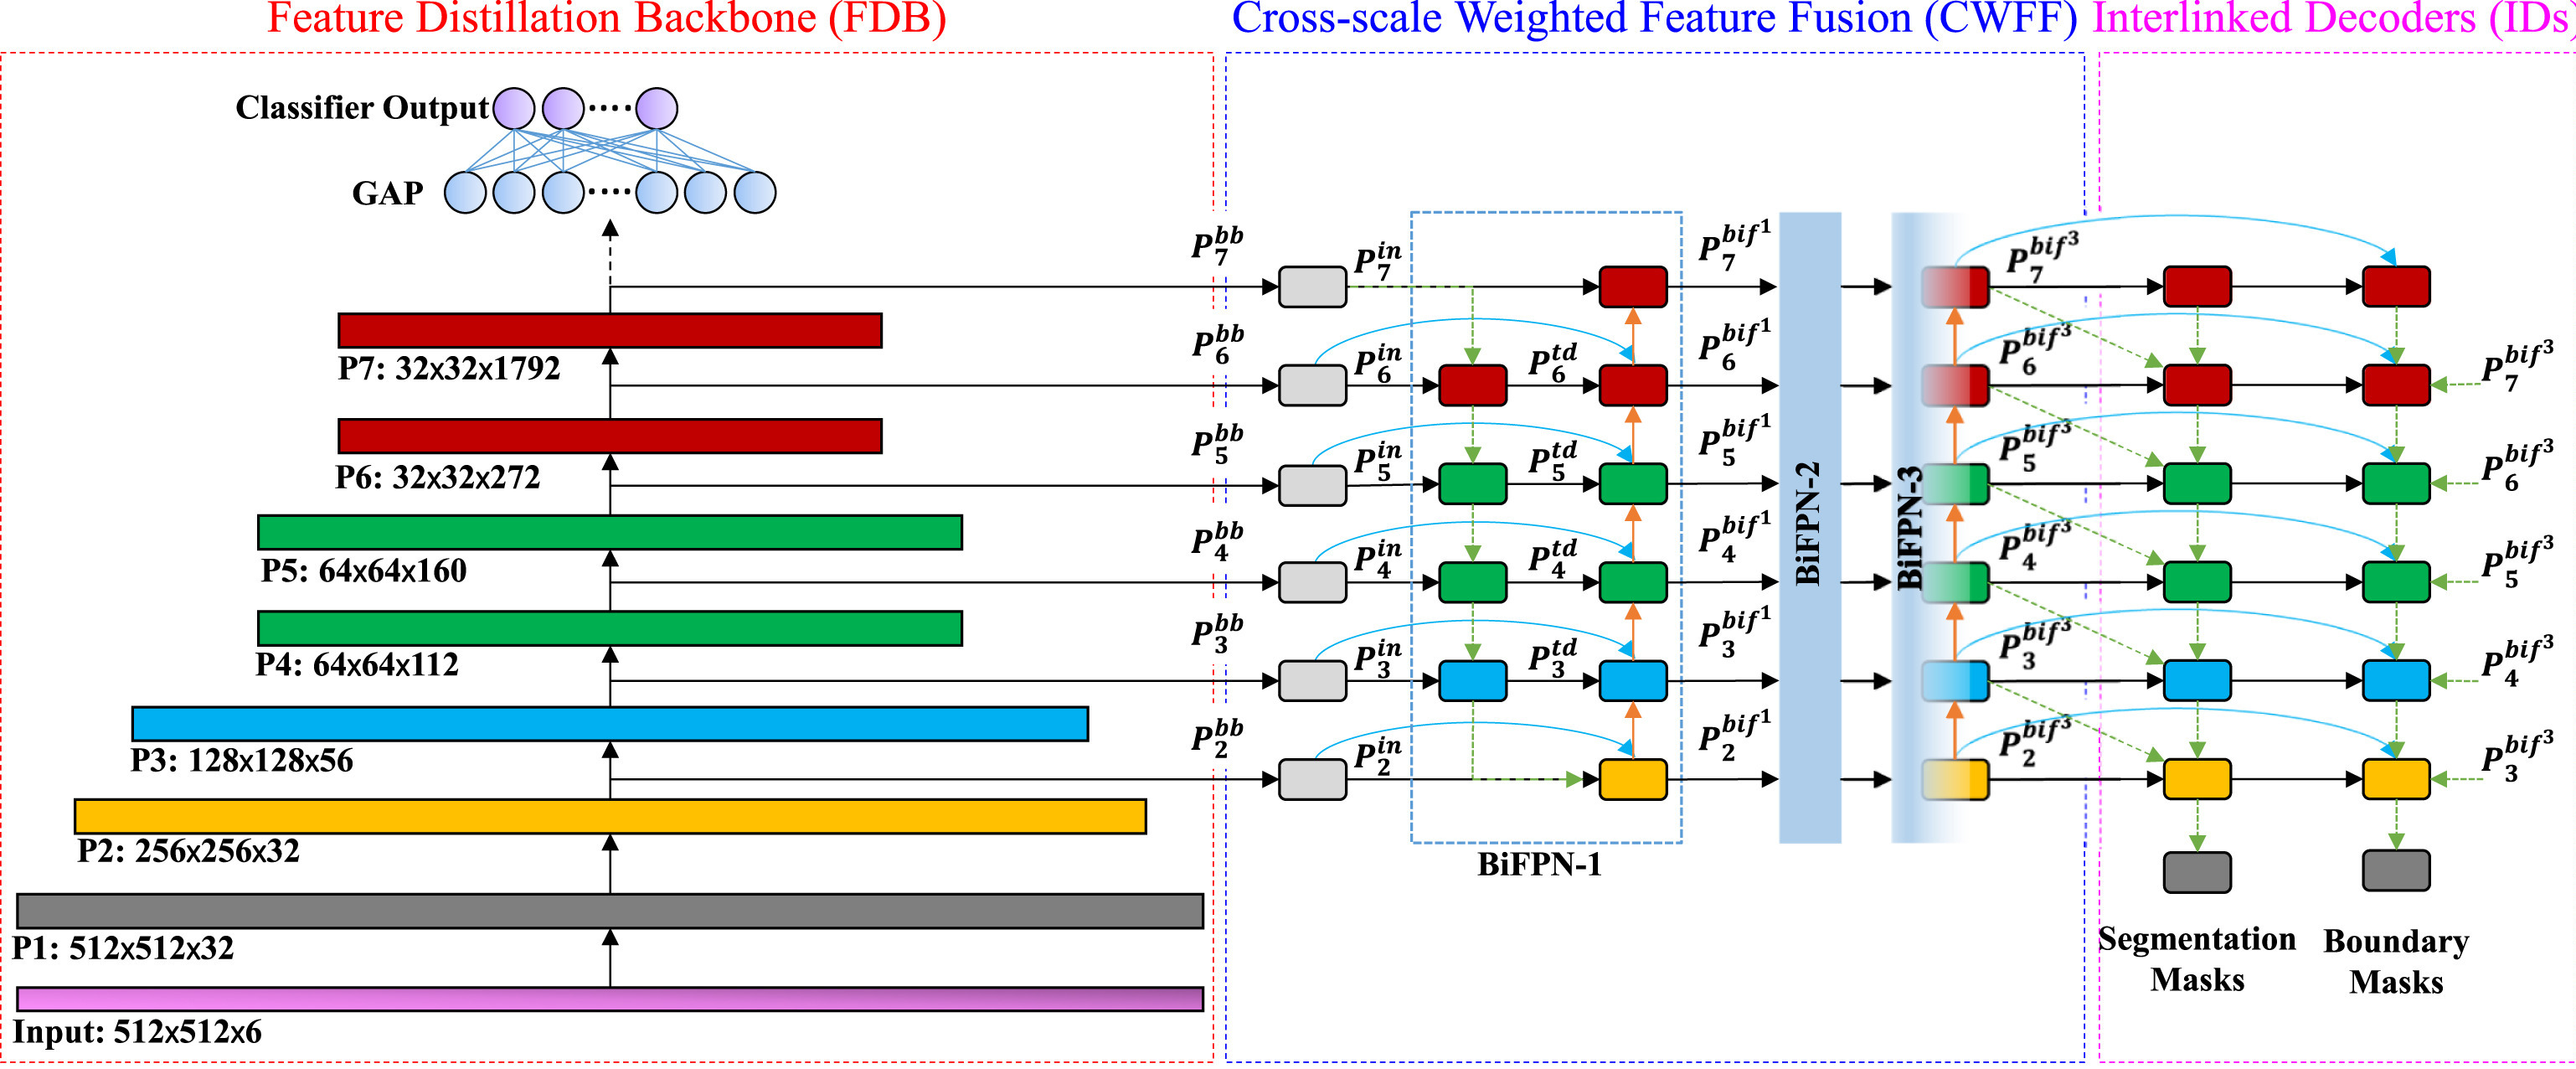
\includegraphics[width=0.7\paperwidth]{img/1-s2.0-S0893608022000612-gr3_lrg-crop.jpg}
       \end{figure}
    \end{frame}

    \begin{frame}{Proposal (I)}
    \textbf{Design and development of an efficient framework for \textit{CBMIR} with}:

    \begin{itemize}
        \item Novel generative neural network for the feature extraction of pap smear images
        \item Optimal retrieval with graph-based nearest neighbour algorithm
    \end{itemize}

    \textbf{Novel generative neural network}
    \begin{itemize}
        \item One big generator: multi-task network for classification and segmentation (semantic and boundary)
        \item Three discriminators
        \item Investigate and analyse the combination of features vectors aimed for a robust and richness embeddings (i e. combs for $F_{I}^{D},F_{SM}^{D},F_{BM}^{D}, F_{backbone}$)
    \end{itemize}

    \textbf{Optimal retrieval}: \textit{HNSW}~\cite{Malkov2016EfficientAR, Boytsov2013EngineeringEA} according to the benchmark of \textit{Aumüller M. et al.}~\cite{10.48550/arxiv.1807.05614}
    
    \end{frame}

    \begin{frame}{Proposal (II)}
        \begin{figure}
        \centering
        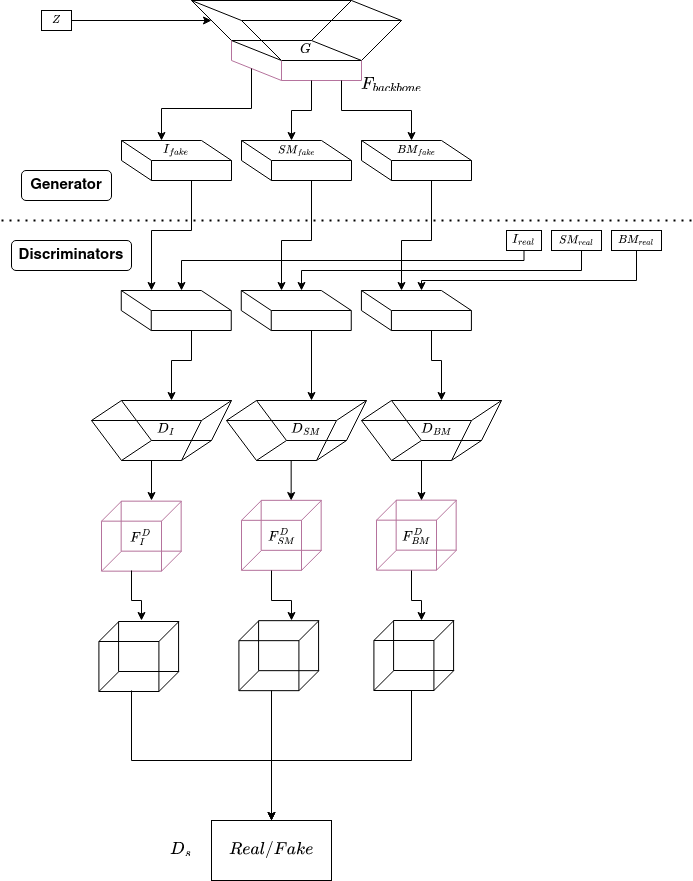
\includegraphics[width=0.8\textwidth]{img/arq-prop.png}
        \end{figure}
    \end{frame}

    \begin{frame}{Hypothesis}
        \begin{tcolorbox}[colback=green!5,colframe=LimeGreen,title=Hypothesis]
        \begin{itemize}
            \item It's possible generate multiples \textit{features vectors} that could be more robust and efficient to be used by a \textit{CMBIR} for pap smear images, using  a generative neural network to classification and segmentation. 
            \item The proposed \textit{CMBIR} is capable of maintain or exceed the time and efficiency in the retrieval of pap smear images with respect to others \textit{CMBIR} of the state of the art.
        \end{itemize}
        \end{tcolorbox}
    \end{frame}

    \begin{frame}{Resources}
    \textbf{Data sets pap smear imgs}
    \begin{itemize}
        \item ISBI Challenges: ISBI 2014 and 2015 challenges dataset with 945 images and 17 images respectively. Included overlapping cells.
        \cite{7005499}\cite{Lu2017}.
        \item Herlev dataset: 917 isolated sigle-cell images~\cite{Marinakis2009}\cite{Dounias2006AutomatedIO}\cite{asljkhdjaskdj}\cite{86c7f5c1a9f84a7484731dd71671c563}.
        \item SIPaKMeD: 4049 isolated sigle-cell images~\cite{8451588}.
        \item liquid-based cytology Pap smear dataset: 963 full images ~\cite{Hussain2020}.
    \end{itemize}\vspace{5mm}

    \textbf{Metrics}
    \begin{itemize}
        \item \textit{CBIR metrics}: precision y recall
        \item \textit{Generated objects}:
        \begin{itemize}
            \item Images: inception score (IS) and Frechet inception distance (FID)
            \item Mask: dice coefficient
        \end{itemize}
    \end{itemize}

    \textbf{Tools}
    \begin{itemize}
        \item \textit{PyTorch}: Network
        \item \textit{HNSW}: Nearest neighbour search
        \item \textit{Django}: Back-end - API REST
    \end{itemize}
    \end{frame}

    \begin{frame}{Extra}
        \begin{center}
            \textbf{Transfer learning with multiple nuclei images}
        \end{center}
        \vspace{10mm}
        \begin{itemize}
            \item Train a backbone with multiple datasets of nuclei images
            \item Use different tissue types
            \begin{itemize}
                \item PanNuke\footnote{\url{https://jgamper.github.io/PanNukeDataset/}}: 205,343 labeled images (19 types)
                \item HoVer-Net\footnote{\url{https://warwick.ac.uk/fac/cross_fac/tia/data/hovernet/}}: 24,319 images
                \item EBHI-Seg\footnote{\url{https://figshare.com/articles/dataset/EBHI-SEG/21540159/1}}: 5,170 images (6 types)
            \end{itemize}
        \end{itemize}
        
    \end{frame}

    \begin{frame}
        \centering
        \Huge Thanks !
    \end{frame}
    
    \begin{frame}[allowframebreaks]{References}
	    \scriptsize
	    \bibliography{report}
        \bibliographystyle{spiebib}
	\end{frame}
     
\end{document}